\chapter{Trabajo realizado}


	%=========================================================
	%                                                         Trabajo realizado
	%=========================================================
	\section{Trabajo realizado}
	Las tareas realizadas para la construcción de RIDESCOM son explicadas a continuación en los SPRINTS 
	
	%=========================================================
	%                                                         Sprint 0
	%=========================================================
	\section{Sprint 0}
	\noindent En este SPRINT se declara el planteamiento y comportamiento de la aplicación como tal, en sus inicios, el plan de desarrollo y los posibles resultados que otorgará.
	Este SPRINT no se contempló en la entrega del protocolo, sin embargo es de importancia ya que en este se definen, las herramientas que se van a emplear, el análisis del sistema, visualizar y proponer el proceso que se emplea.
	También se especificará cómo es que se instalaron las herramientas que se emplearon.
	
	\begin{enumerate}
		\item Base de Datos
		A continuación se mostrará la estructura que tendrá la Base de Datos de la aplicación.
		\begin{figure}[hbt!]
			\centering
			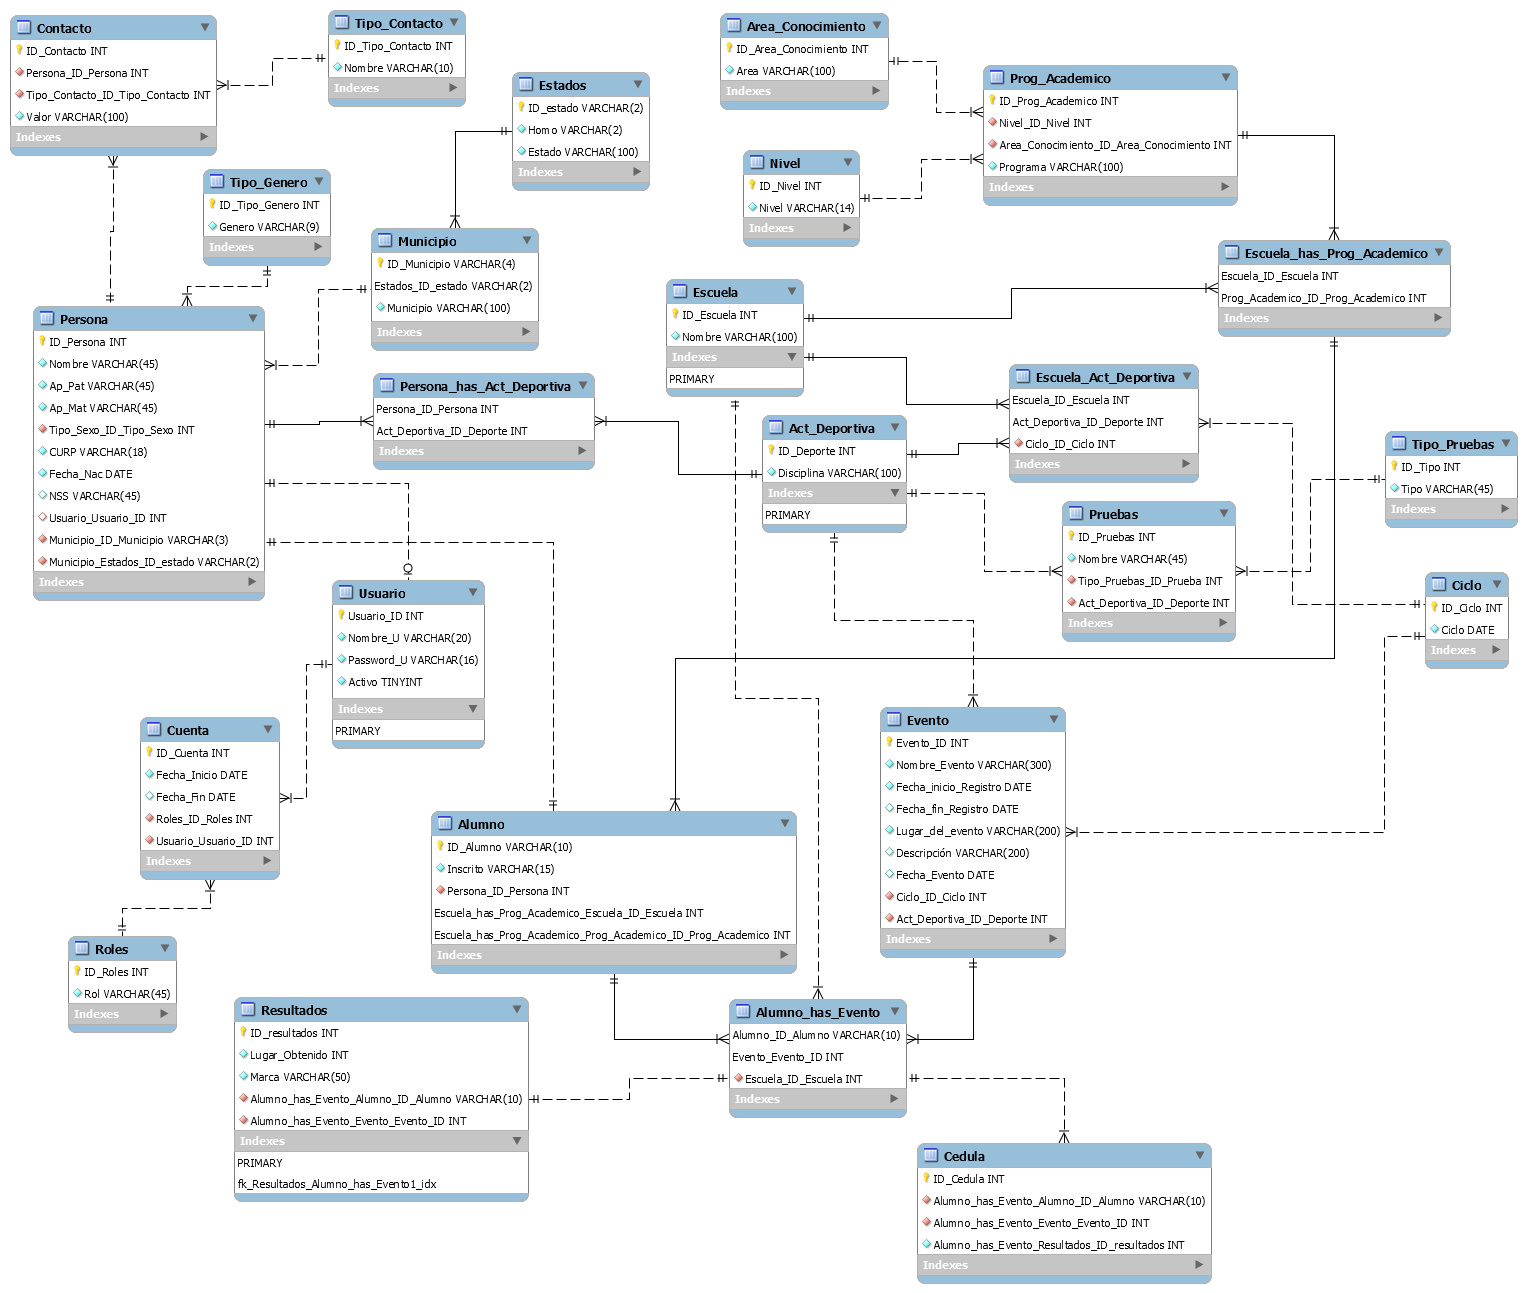
\includegraphics[width=22cm, height=15cm, angle=90]{Imagenes/BasedeDatos.png}
			\caption{Base de Datos}
		\end{figure}
	\end{enumerate}
	\pagebreak
	
	Como parte de la notación que se empleó 
	
	%=========================================================
	%                                                         Sprint 1
	%=========================================================
	\section{Sprint 1}
	\noindent El desarrollo de este SPRINT se consideró que la manera de validación del participante será que el alumno que desee participar en un evento interpolitécnico para ello deberá registrarse en la aplicación web posteriormente, deberá acudir con el coordinador de su Unidad Académica y que el corrobore sus datos solicitando alguna identificación, cabe destacar que este proceso de validación se hará solo una vez.
	Una vez que haya sido validado por el coordinador y este, activará su cuenta, el alumno interesado podrá ingresar en el sistema e inscribirse en una evento interpolitécnico dentro de las fechas establecidas.
	El objetivo de este mecanismo es comprobar la existencia de un alumno en la base de datos del plantel o en el IPN y aceptar únicamente a los que estén inscritos.
	
	
	%=========================================================
	%                                                         Sprint 2
	%=========================================================
	\section{Sprint 2}
	\noindent Para la desarrollo de este SPRINT se tomaron los debidos requerimientos para la realización del diseño de las interfaces y así hacer que la aplicación sea amigable con el usuario utilizando las siguientes plantillas para la visualización de las interfaces como una propuesta.
	
	\noindent Interfaz Inicio general: Esta interfaz es la principal donde los usuarios podrán visualizar datos de aspecto público. \newline
	Parte 1:
	Cualquier usuario que visite la URL de la aplicación podrá ver los elementos de navegación tales como: Inicio (Página principal), Registro, Calendario, Inicia Sesión, Contacto, los deportes que se imparten en la ESCOM, una introducción a los eventos interpolitécnicos deportivos próximos, como se muetra en la Figura 14. 
	\begin{figure}[hbt!]
		\centering
		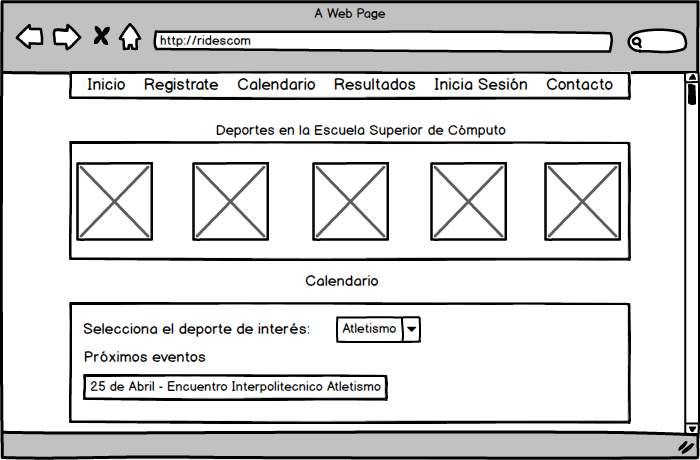
\includegraphics[width=10cm, height=6cm]{Imagenes/Disenos/p19Iniciogeneral.png}
		\caption{Página Inicio (comunidad en general)}
	\end{figure}
	\pagebreak
	Parte 2:
	Dentro de la misma habrá una sección de resultados generales de los últimos eventos realizados y finalmente una  sección donde se localiza el contacto del plantel para más información al respecto y un contacto de Facebook del área de actividades deportivas de la ESCOM, como se muetra en la Figura 15.
	\begin{figure}[hbt!]
		\centering
		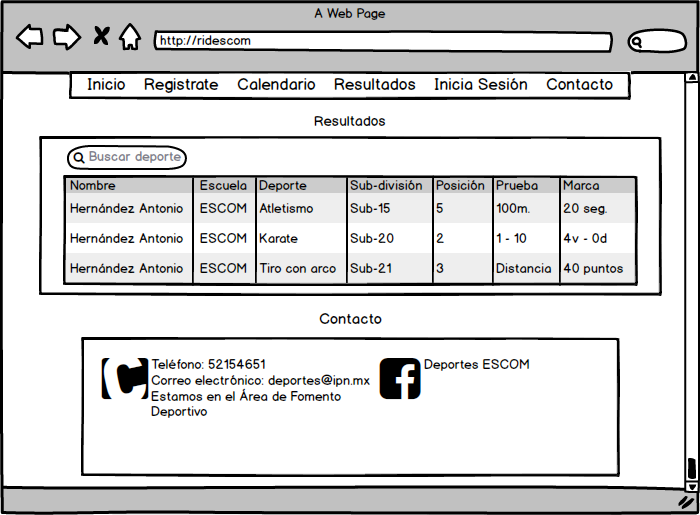
\includegraphics[width=10cm, height=6cm]{Imagenes/Disenos/p20Iniciogeneral1.png}
		\caption{Página Inicio 2 (comunidad en general)}
	\end{figure}
	
	\noindent Interfaz Login del Jefe del Departamento de Fomento Deportivo: En esta interfaz ayuda al usuario indicando los elementos que se necesitan para iniciar sesión como usuario de la aplicación (Nombre-Usuario/contraseña previamente registrado), si el usuario no existe el mecanismo realizado en el SPRINT1 se encargará de rechazarlo, podrá recuperar su contraseña en la sección de “¿Olvidaste tu contraseña?”, como se muestra en la Figura 20.\pagebreak
	\begin{figure}[hbt!]
		\centering
		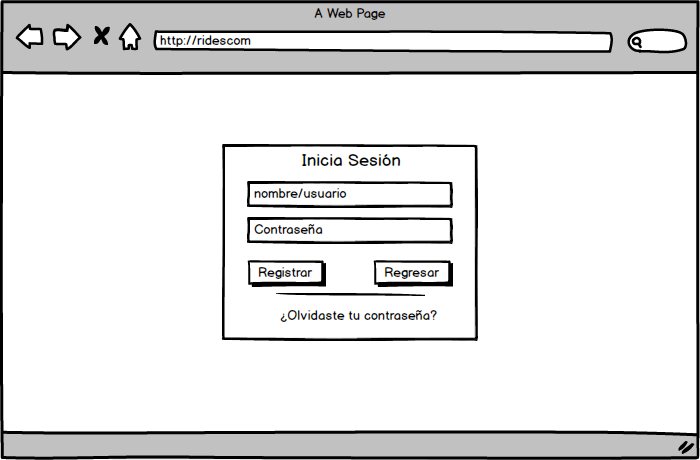
\includegraphics[width=10cm, height=6cm]{Imagenes/Disenos/p2LoginJFD.png}
		\caption{Login del Jefe del Departamento de Fomento Deportivo}
	\end{figure}
	
	\noindent Interfaz Inicio del Jefe del Departamento de Fomento Deportivo: El diseño de la página será muy similar con el resto de los usuarios, sin embargo, este contará con distintas opciones como son: Crear un evento deportivo, Resultados, Calendario y Control de cordinadores donde en este apartado tendrá la opción de Consultar coordinadores, Registrar usuario, Modificar contraseña de los coordinadores de las Unidades Académicas, como se muestra en la Figura 22. El diseño en general de la vista de este usuario se puede ver en  las Figuras 21 y 23.
	\begin{figure}[hbt!]
		\centering
		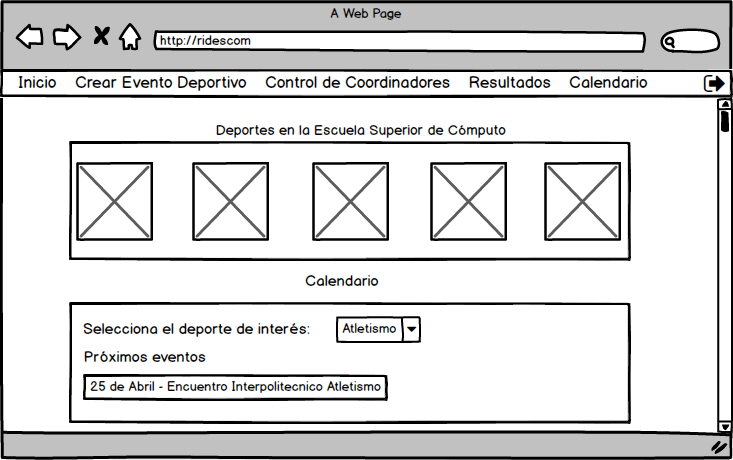
\includegraphics[width=10cm, height=6cm]{Imagenes/Disenos/p3InicioJefeFD.png}
		\caption{Página principal Jefe del Departamento de Fomento Deportivo}
	\end{figure}
	
	\pagebreak
	
	\begin{figure}[hbt!]
		\centering
		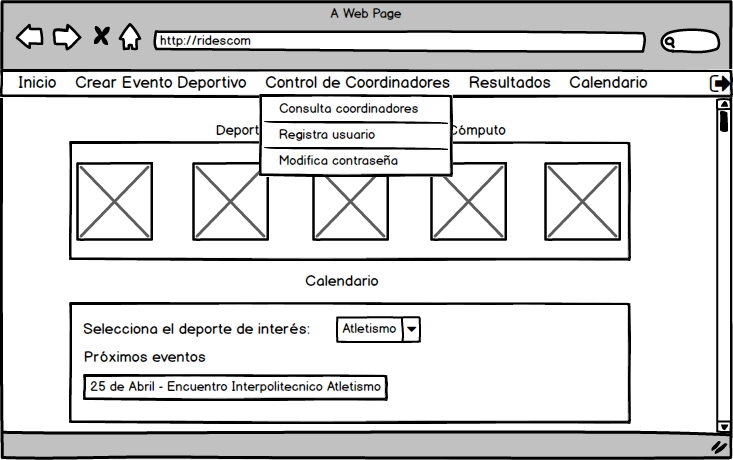
\includegraphics[width=10cm, height=6cm]{Imagenes/Disenos/p4InicioJefeFDopcipones.png}
		\caption{Página principal Jefe del Departamento de Fomento Deportivo}
	\end{figure}
	\begin{figure}[hbt!]
		\centering
		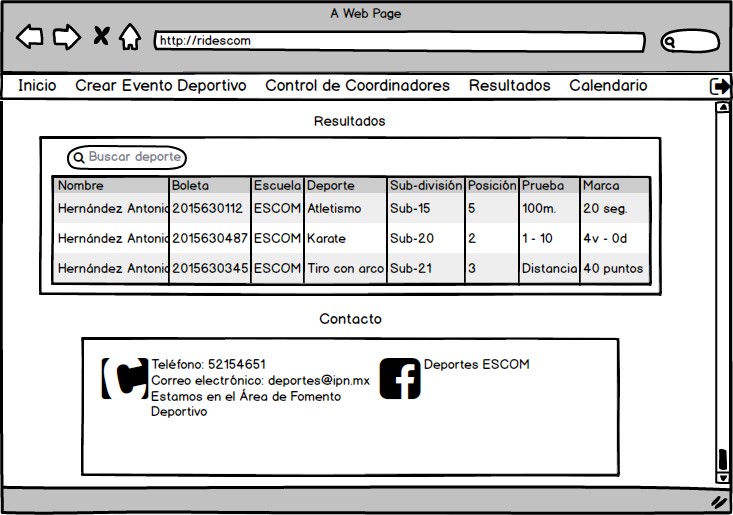
\includegraphics[width=10cm, height=6cm]{Imagenes/Disenos/p5InicioJefeFD1.png}
		\caption{Página principal del Jefe del Departamento de Fomento Deportivo 1}
	\end{figure}
	
	\noindent Interfaz Crear un evento interpolitécnico: Dentro de esta vista el Jefe del Departamento de Fomento Deportivo llenaráa los campos para poder dar de alta algún evento, se pedirá el Nombre del evento, Fecha en la que se llevará acabo, Fecha inicio de inscripción y Fecha fin de inscripción, un campo de Descripción donde podrá agregar la dirección del lugar entre otros datos. Se seleccionará el deporte al que corresponde dicho evento, así como la Sub-división y Prueba, como se muestra en la Figura 24.
	\pagebreak
	\begin{figure}[hbt!]
		\centering
		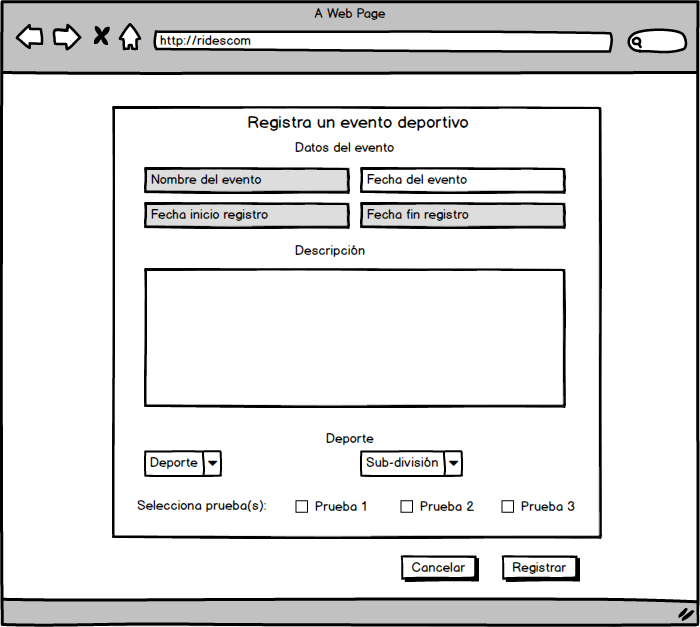
\includegraphics[width=10cm, height=6cm]{Imagenes/Disenos/p6Creareventodeportivo.png}
		\caption{Crear un evento deportivo}
	\end{figure}
	
	\noindent Interfaz Registra un coordinador: Se solicitarán datos como Nombre, Apellido Paterno, Apellido Materno,correo electrónico, teleéfonos de contacto y Escuela a la que pertenece, como se muestra en la Figura 25.
	\begin{figure}[hbt!]
		\centering
		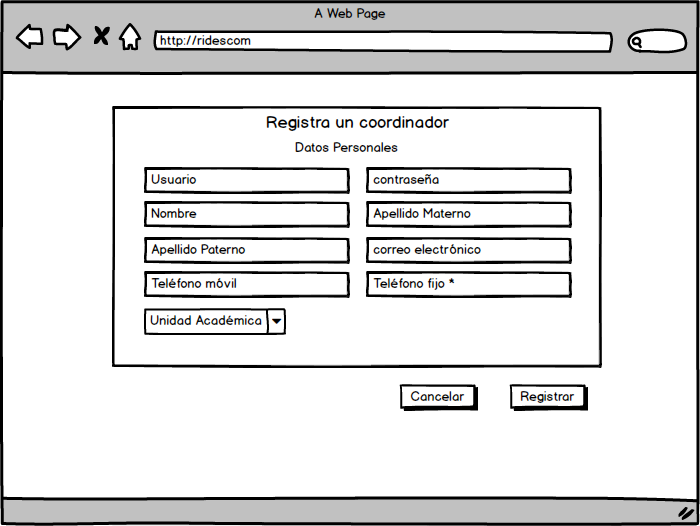
\includegraphics[width=10cm, height=6cm]{Imagenes/Disenos/p7Registrocoordinador.png}
		\caption{Registra un coordinador}
	\end{figure}
	
	\noindent Interfaz login coordinador: En esta interfaz ayuda al usuario indicando los elementos que se necesitan para iniciar sesión como usuario de la aplicación (Nombre-Usuario/contraseña previamente registrado), si el usuario no existe el mecanismo realizado en el SPRINT1 se encargará de rechazarlo, como se muestra en la Figura 26. En caso de que el coordinador olvide su contraseña deberá ponerse en contacto con el Jefe del Departamento de Fomento Deportivo para solicitar el cambio de contraseña \pagebreak
	\begin{figure}[hbt!]
		\centering
		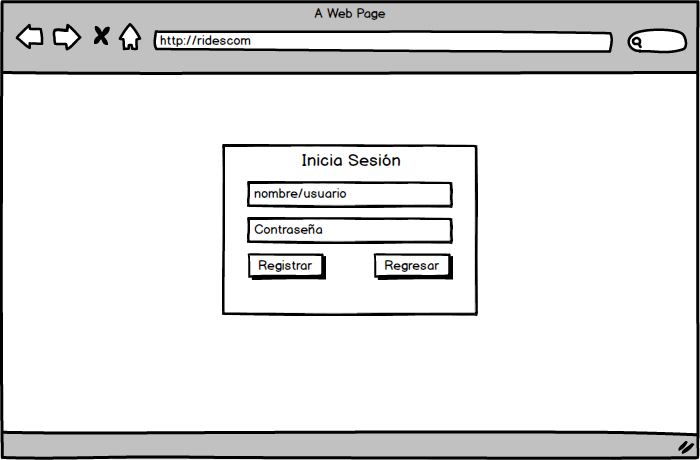
\includegraphics[width=10cm, height=6cm]{Imagenes/Disenos/p8LogincoordUA.png}
		\caption{Login para el coordinador de la Unidad Académica}
	\end{figure}
	
	\noindent Interfaz  Inicio del coordinador de una Unidad Académica: Al igual que el resto de los usuarios en general tiene un diseño muy similar, la diferencia recae en las opciones que puede realizar, en este caso son: Registrar entrenador, Calendario, Resultados, Consulta de inscripciones y Válidar perfil, como se muestra en las Figura 27 y en la Figura 28 se puede observar que estará disponible un apartado para publicar algun evento previamente dado de alta en la red social de Facebook.
	
	\begin{figure}[hbt!]
		\centering
		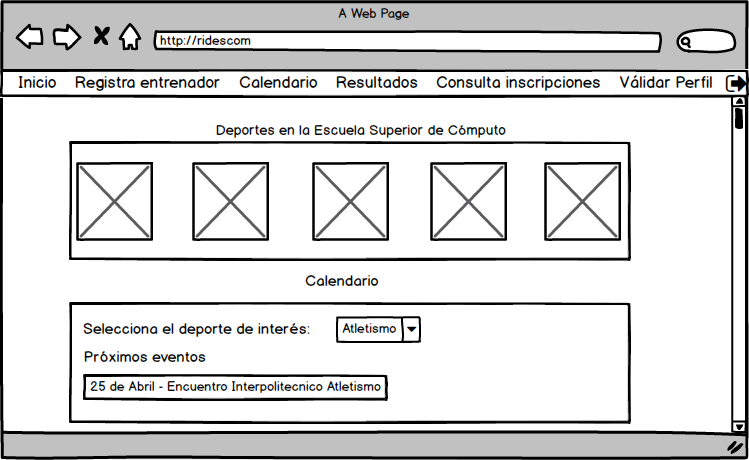
\includegraphics[width=10cm, height=6cm]{Imagenes/Disenos/p9InicioCoordUA.png}
		\caption{Página principal del coordinador de la Unidad Académica}
	\end{figure}
	
	\pagebreak
	
	\begin{figure}[hbt!]
		\centering
		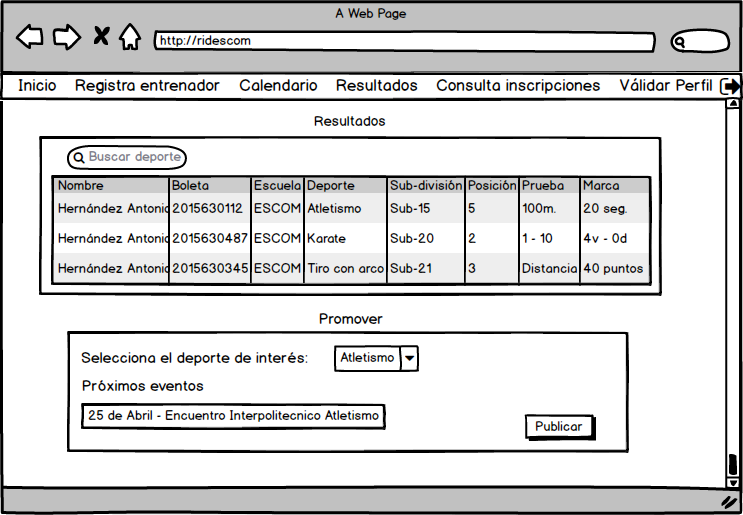
\includegraphics[width=10cm, height=6cm]{Imagenes/Disenos/p10InicioCoordUA1.png}
		\caption{Página principal del coordinador de la Unidad Académica 1}
	\end{figure}

	\noindent Interfaz Resultados: Este módulo esta designado para que se ingresen los resultados de los participantes y sean vistos en la página principal. Podrá ingresar hasta 20 datos por vez, como se muestra en la Figura 31.
	\begin{figure}[hbt!]
		\centering
		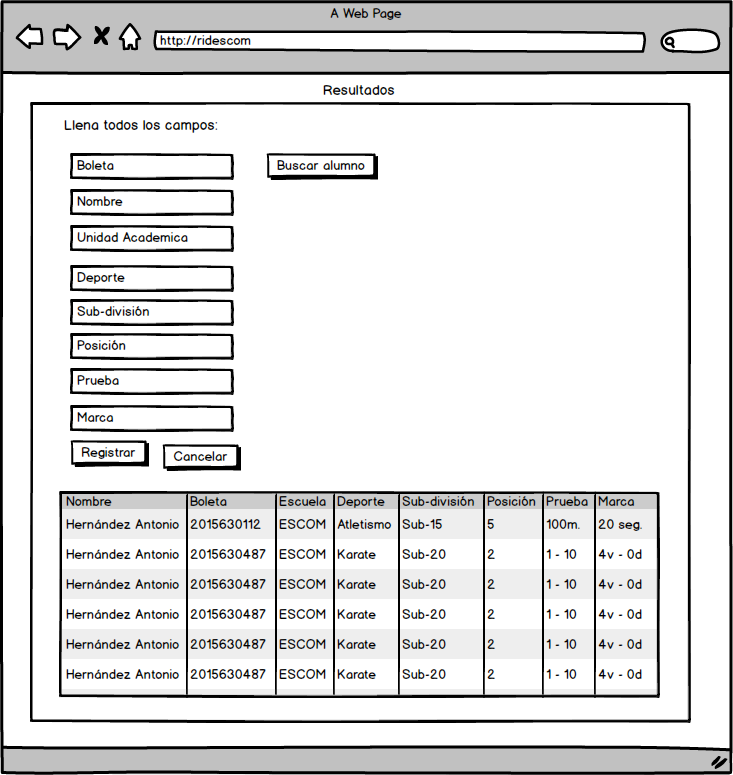
\includegraphics[width=10cm, height=6cm]{Imagenes/Disenos/p11Ingresaresultados.png}
		\caption{Ingresa resultados de los eventos}
	\end{figure}
	
	\noindent Interfaz Registro entrenador: En este  módulo el coordinador deberá los campos solicitados tales como: No. Empleado, Nombre, Apellidos, Correo electrónico, Teléfono fijo, Teléfono móvil, asi como definir a que deporte pertenece y por ultimo, especificar si cuenta con un asistente, como se muestra en la Figura 29.
	\begin{figure}[hbt!]
		\centering
		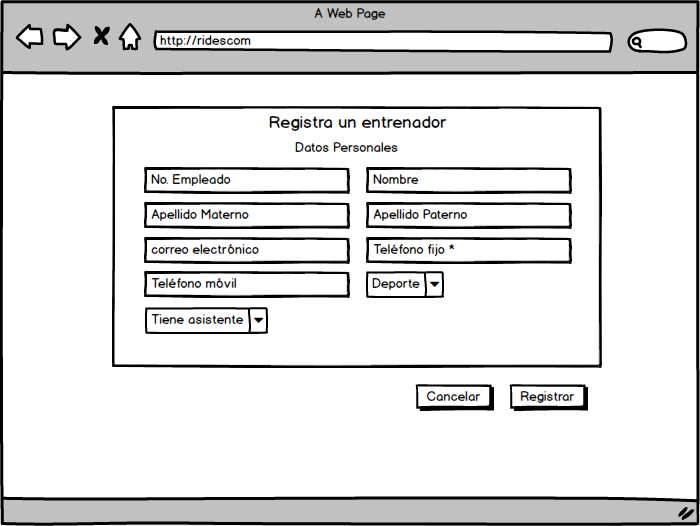
\includegraphics[width=10cm, height=6cm]{Imagenes/Disenos/p12Registroentrenador.png}
		\caption{Registra un entrenador}
	\end{figure}
	\pagebreak
	
	\noindent Interfaz Login alumno: En esta interfaz ayuda al usuario indicando los elementos que se necesitan para iniciar sesión como usuario de la aplicación (Usuario/contraseña previamente registrado), si el usuario no existe el mecanismo realizado en el SPRINT1 se encargará de rechazarlo, podrá recuperar su contraseña en la sección de “¿Olvidaste tu contraseña?”, como se muestra en la Figura 16. \pagebreak
	\begin{figure}[hbt!]
		\centering
		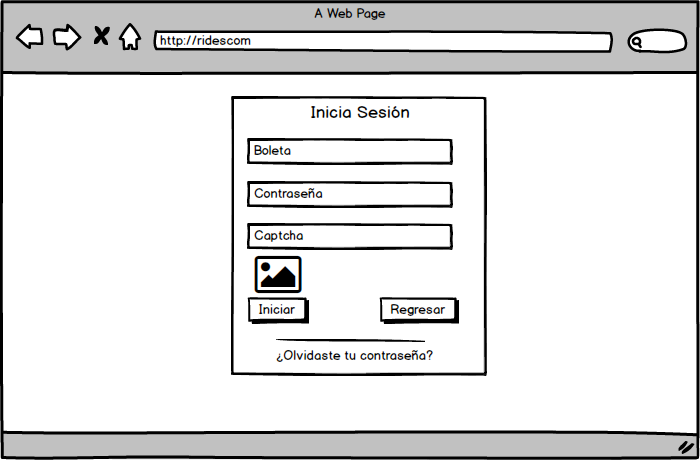
\includegraphics[width=10cm, height=6cm]{Imagenes/Disenos/p1Login.png}
		\caption{Login}
	\end{figure}

	\noindent Interfaz Inicio del alumno: El diseño de la página será muy similar con el resto de los usuarios, sin embargo, este contará con distintas opciones como son: Inscribir un Interpolitécnico, Calendario, Consulta tus registros y Contacto, como se muestra en la Figura 21. El diseño en general de la vista de este usuario se puede ver en  las Figuras 32 y 33.
	\begin{figure}[hbt!]
		\centering
		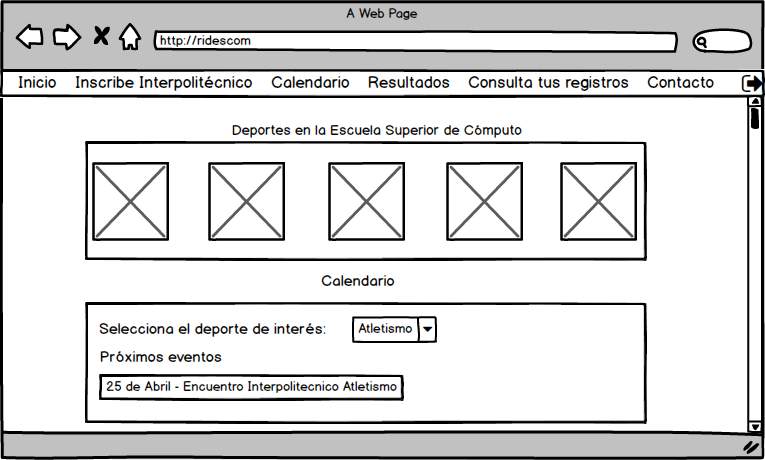
\includegraphics[width=10cm, height=6cm]{Imagenes/Disenos/p13Iniciopaticipante.png}
		\caption{Página principal del participante}
	\end{figure}
	\begin{figure}[hbt!]
		\centering
		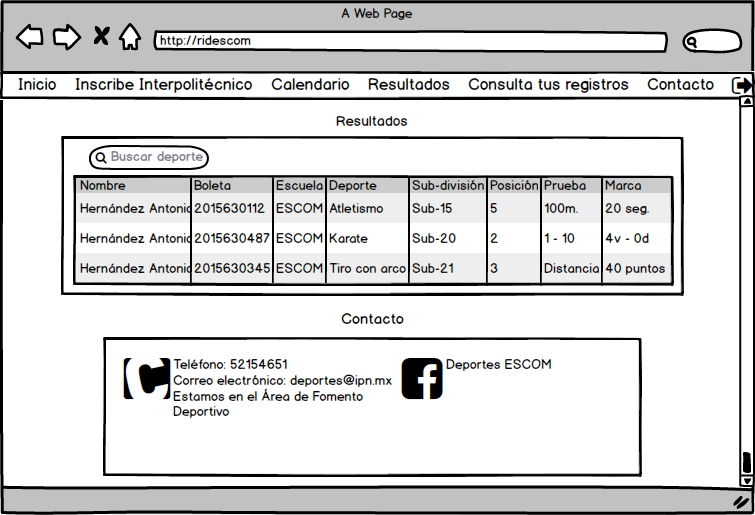
\includegraphics[width=10cm, height=6cm]{Imagenes/Disenos/p14Iniciopaticipante1.png}
		\caption{Página principal del participante 1}
	\end{figure}
	
	\noindent Interfaz Inscribir interpolitécnico: En este módulo el alumno primero deberá válidar el estatus de su inscripción, si esta inscrito en el periodo actual, se habilitará el botón para registrar la cédula. En caso contrario el botón no estará habilitado y por tanto, no podrá inscribirse. Los campos que debera llenar el alumno serán: Grupo, NSS (Número de Seguro Social), Lugar de Nacimiento, correo electrónico, Delegación/Municipio, asi como seleccionar el deporte, sub-division y prueba en la que quiere participar, como se muestra en la Figura 34.
	\begin{figure}[hbt!]
		\centering
		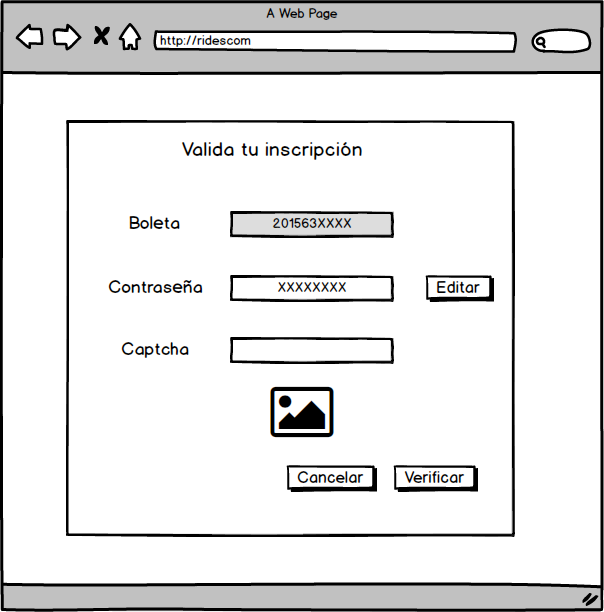
\includegraphics[width=10cm, height=6cm]{Imagenes/Disenos/p15InscripcionInterpolitecnico1.png}
		\caption{Inscribir un interpolitécnico}
	\end{figure}

	\begin{figure}[hbt!]
	\centering
	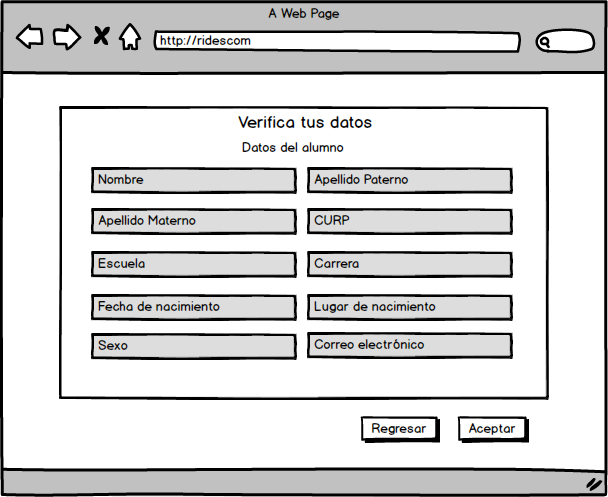
\includegraphics[width=10cm, height=6cm]{Imagenes/Disenos/p16InscripcionInterpolitecnico2.png}
	\caption{Inscribir un interpolitécnico}
	\end{figure}

	\begin{figure}[hbt!]
	\centering
	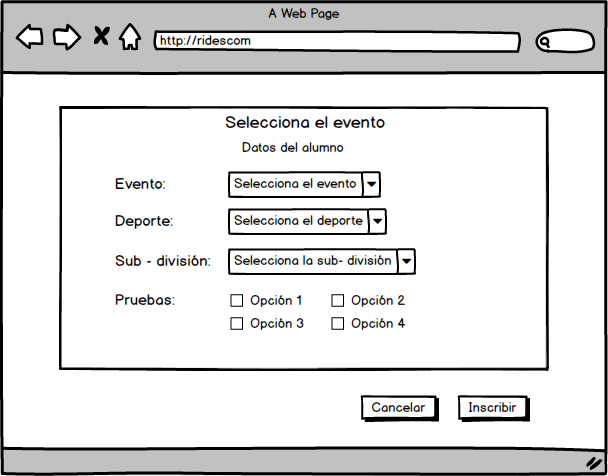
\includegraphics[width=10cm, height=6cm]{Imagenes/Disenos/p17InscripcionInterpolitecnico3.png}
	\caption{Inscribir un interpolitécnico}
	\end{figure}
	\pagebreak
	
	\noindent Interfaz Consulta tus registros: En este módulo, el participante podrá visualizar en una tabla los eventos a los cuales se a registrado, a su vez le mostrará información como: el deporte, prueba Fecha del Evento y la direccion del mismo, como se muestra en la Figura 35.
	\begin{figure}[hbt!]
		\centering
		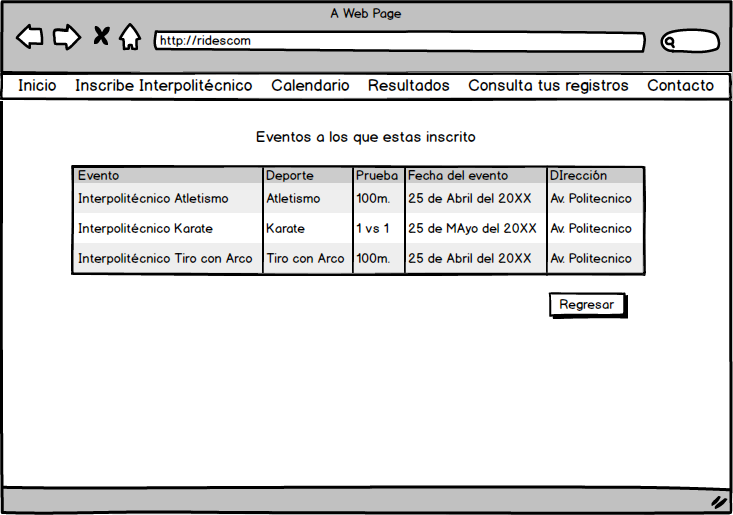
\includegraphics[width=10cm, height=6cm]{Imagenes/Disenos/p18ConsultaInscripciones.png}
		\caption{Consulta eventos a los que se ha registrado}
	\end{figure}
	%=========================================================
	%                                                         Sprint 3
	%=========================================================
	\section{Sprint 3}
	
	%=========================================================
	%                                                         Sprint 4
	%=========================================================
	\section{Sprint 4}
	
	%=========================================================
	%                                                         Sprint 5
	%=========================================================
	\section{Sprint 5}
	
	%=========================================================
	%                                                         Sprint 6
	%=========================================================
	\section{Sprint 6}
	
	%=========================================================
	%                                                         Sprint 7
	%=========================================================
	\section{Sprint 7}
